\documentclass[12pt]{article}

\usepackage{hcmus-report-template}

% Disable indentation on new paragraphs
\setlength{\parindent}{0pt}

% Line spacing 1.5
\renewcommand{\baselinestretch}{1.5}

% Optional: graphic path
% \graphicspath{PATH_TO_GRAPHIC_FOLDER}

% To use Times font family, uncomment this row
% \usepackage{mathptmx}

% To use roman section / subsection, uncomment these rows
% \renewcommand{\thesection}{\Roman{section}}
% \renewcommand{\thesubsection}{\thesection.\Roman{subsection}}

% Define course name, report name and report title.
\newcommand{\coursename}{Nhập môn Xử lí Ngôn ngữ Tự nhiên}
\newcommand{\reportname}{Fine-tuning mô hình DeepSeek-OCR cho bài toán nhận diện chữ viết tay tiếng Việt}
\newcommand{\reporttitle}{Project \#2   }

\newcommand{\studentname}{Nguyễn Thiên Ấn - 23122020}
\newcommand{\teachername}{PGS.TS. Đinh Điền \\ TS. Nguyễn Hồng Bửu Long}

% Header
\lhead{\reporttitle}
\rhead{
Trường Đại học Khoa học Tự nhiên - ĐHQG HCM\\
\coursename
}


% ============ DOCUMENT ============
\begin{document}

\pagenumbering{roman}
\input{content/title.tex}

\tableofcontents
\pagebreak

\pagenumbering{arabic}
\setcounter{page}{1}

\section{Bối cảnh}

Nhận dạng ký tự quang học (Optical Character Recognition - OCR) là công nghệ cho phép chuyển đổi văn bản dưới dạng hình ảnh thành dữ liệu số có thể chỉnh sửa và tìm kiếm. Đây là thành phần quan trọng trong quá trình số hóa tài liệu và tự động hóa quy trình xử lý thông tin.

\subsection{Thực trạng hiện tại}

Lĩnh vực OCR đã trải qua sự chuyển dịch mạnh mẽ từ các phương pháp so khớp mẫu truyền thống sang các kiến trúc học sâu (Deep Learning) hiện đại. Các hệ thống truyền thống dựa trên trích xuất đặc trưng thủ công thường gặp khó khăn với nhiễu và biến dạng. Sự ra đời của Mạng nơ-ron Tích chập (CNN) và Mạng nơ-ron Hồi quy (RNN/LSTM) đã giải quyết tốt vấn đề này, cải thiện đáng kể khả năng nhận dạng chuỗi ký tự.

Gần đây, kiến trúc Transformer với cơ chế Self-Attention đang dần thay thế RNN, cho phép nắm bắt ngữ cảnh toàn cục tốt hơn và xử lý hiệu quả các cấu trúc văn bản phức tạp thông qua các mô hình Vision-Language như Donut hay TrOCR.

\subsection{OCR cho tiếng Việt}

Mặc dù đạt độ chính xác cao trên các ngôn ngữ Latinh cơ bản, việc áp dụng OCR cho tiếng Việt vẫn gặp nhiều thách thức do đặc điểm ngôn ngữ \cite{le2025surveyvietnamesedocumentanalysis}:

\begin{itemize}
    \item \textbf{Vấn đề mất dấu:} Tiếng Việt có hệ thống dấu thanh và dấu phụ dày đặc, nhiều dấu chiếm diện tích rất nhỏ. Các kiến trúc CNN tiêu chuẩn sử dụng lớp Pooling để giảm chiều dữ liệu thường làm mất các đặc trưng chi tiết này, dẫn đến các lỗi nhầm lẫn phổ biến (ví dụ: "a", "á", "à", "ạ").
    \item \textbf{Sự khan hiếm dữ liệu:} Tài nguyên dữ liệu huấn luyện chất lượng cao cho tiếng Việt, đặc biệt là chữ viết tay tự do và tài liệu lịch sử, còn hạn chế so với tiếng Anh hay tiếng Trung. Các bộ dữ liệu hiện có như VNOnDB hay UIT-HWDB thường có quy mô nhỏ hoặc là dữ liệu tổng hợp, gây khó khăn cho việc huấn luyện các mô hình Deep Learning lớn.
\end{itemize}

Hiện nay, các giải pháp OCR cho tiếng Việt chủ yếu bao gồm:

\begin{itemize}
    \item \textbf{Tesseract OCR:} Hỗ trợ tiếng Việt qua mô hình LSTM nhưng thường có tỷ lệ lỗi ký tự (CER) cao với ảnh nhiễu hoặc bố cục phức tạp.
    \item \textbf{PaddleOCR và VietOCR:} Các phương pháp tiên tiến (SOTA) hiện nay. PaddleOCR (kiến trúc PP-OCR) và VietOCR (dựa trên Transformer) xử lý tốt văn bản nghiêng, cong và giảm thiểu lỗi dấu nhờ cơ chế Attention.
    \item \textbf{Hậu xử lý bằng LLM:} Xu hướng tích hợp Mô hình Ngôn ngữ Lớn (LLM) để hậu xử lý kết quả OCR. LLM tận dụng ngữ cảnh để sửa lỗi chính tả và dấu thanh, đặc biệt hiệu quả với tài liệu cũ hoặc mờ.
\end{itemize}

Tóm lại, bài toán OCR tiếng Việt đang chuyển dịch từ nhận dạng ký tự đơn lẻ sang hiểu tài liệu toàn diện (Document Understanding) và kết hợp đa mô hình để giải quyết vấn đề dấu thanh và cấu trúc phức tạp.
\section{Phương pháp nghiên cứu}

Phần này trình bày chi tiết về dữ liệu và phương pháp tiếp cận được sử dụng trong nghiên cứu. Chúng tôi tập trung phân tích đặc điểm của bộ dữ liệu chữ viết tay tiếng Việt và mô tả kiến trúc mô hình cũng như kỹ thuật tinh chỉnh được áp dụng.

\subsection{Dữ liệu nghiên cứu}

\subsubsection{Bộ dữ liệu UIT-HWDB}
Nghiên cứu sử dụng bộ dữ liệu UIT-HWDB \cite{DBLP:conf/rivf/NguyenVN22} (University of Information Technology - Handwritten Database), một nguồn tài nguyên quan trọng cho cộng đồng nghiên cứu nhận dạng chữ viết tay tiếng Việt. Đây là bộ dữ liệu được thu thập từ chữ viết tay của nhiều người viết khác nhau, đảm bảo tính đa dạng về phong cách viết, nét bút và công cụ viết.

Đặc điểm nổi bật của dữ liệu này là sự hiện diện dày đặc của các ký tự có dấu trong tiếng Việt. Khác với tiếng Anh, tiếng Việt có hệ thống dấu thanh (sắc, huyền, hỏi, ngã, nặng) và dấu mũ (â, ê, ô, ă, ư, ơ) phức tạp. Việc nhận dạng chính xác các dấu này là thách thức lớn nhất, vì chúng thường nhỏ và dễ bị nhầm lẫn hoặc mất mát trong quá trình xử lý ảnh.

Trong phạm vi nghiên cứu này, chúng tôi tập trung vào bài toán nhận dạng ở cấp độ từ (word-level), sử dụng tập dữ liệu con chứa các ảnh từ đơn lẻ được cắt ra từ các dòng văn bản viết tay.

\subsubsection{Tiền xử lý dữ liệu}
Để đảm bảo chất lượng đầu vào cho mô hình, quy trình tiền xử lý được thực hiện qua các bước sau:

\begin{itemize}
    \item \textbf{Chuyển đổi không gian màu:} Ảnh gốc được chuyển đổi sang ảnh xám (grayscale). Bước này giúp loại bỏ nhiễu màu sắc không cần thiết, giảm chiều dữ liệu và tập trung vào thông tin cường độ sáng (intensity) thể hiện nét chữ.
    \item \textbf{Chuẩn hóa (Normalization):} Giá trị pixel của ảnh được chuẩn hóa về khoảng [0, 1] thông qua phương pháp Min-Max. Việc này giúp đồng bộ hóa phân phối dữ liệu, hỗ trợ quá trình hội tụ của mô hình diễn ra nhanh và ổn định hơn.
    \item \textbf{Đồng bộ kích thước:} Các ảnh đầu vào có kích thước không đồng nhất được thay đổi (resize) về một kích thước chuẩn (128x128 pixel). Việc này là cần thiết để đóng gói dữ liệu thành các batch trong quá trình huấn luyện.
\end{itemize}

\subsubsection{Phương pháp lấy mẫu dữ liệu (Data Sampling)}

Để đảm bảo tính khách quan và độ tin cậy của kết quả đánh giá, ta sử dụng phương pháp \textbf{Lấy mẫu ngẫu nhiên đơn giản (Simple Random Sampling)} để phân chia dữ liệu. Toàn bộ tập dữ liệu sau khi tiền xử lý được xáo trộn ngẫu nhiên và chia thành ba tập con độc lập theo tỷ lệ:
\begin{itemize}
    \item \textbf{Tập huấn luyện (Training set - 80\%):} Dùng để cập nhật trọng số mô hình.
    \item \textbf{Tập thẩm định (Validation set - 10\%):} Dùng để tinh chỉnh siêu tham số và đánh giá sớm (early stopping).
    \item \textbf{Tập kiểm tra (Test set - 10\%):} Dùng để đánh giá hiệu năng cuối cùng của mô hình.
\end{itemize}
Việc phân chia ngẫu nhiên giúp đảm bảo phân phối của các ký tự và kiểu chữ trong ba tập là tương đồng nhau, tránh hiện tượng thiên lệch (bias).

\subsection{Mô hình và Kỹ thuật huấn luyện}

\subsubsection{Kiến trúc Vision-Language}
Chúng tôi tiếp cận bài toán OCR dưới góc độ của một bài toán đa phương thức (Multimodal), sử dụng mô hình nền tảng là DeepSeek-OCR (dựa trên kiến trúc Qwen-VL) \cite{unsloth2025deepseek}. Thay vì sử dụng các kiến trúc CNN-RNN truyền thống, mô hình này kết hợp một bộ mã hóa hình ảnh (Vision Encoder) mạnh mẽ với một mô hình ngôn ngữ lớn (Large Language Model - LLM).

Ưu điểm của phương pháp này là khả năng tận dụng tri thức ngôn ngữ phong phú của LLM để giải quyết các trường hợp chữ viết mờ, khó đọc hoặc bị che khuất, dựa trên ngữ cảnh của các ký tự xung quanh.

\subsubsection{Kỹ thuật Fine-tuning}
Để thích nghi mô hình với miền dữ liệu chữ viết tay tiếng Việt mà không tốn kém quá nhiều tài nguyên tính toán, chúng tôi sử dụng kỹ thuật \textbf{LoRA (Low-Rank Adaptation)} và thư viện Unsloth \cite{unsloth_library} để tối ưu hóa quá trình huấn luyện.

LoRA cho phép đóng băng các trọng số của mô hình tiền huấn luyện khổng lồ và chỉ cập nhật các ma trận phân rã hạng thấp (low-rank decomposition matrices) được thêm vào các lớp Attention. Phương pháp này giúp giảm đáng kể số lượng tham số cần huấn luyện trong khi vẫn duy trì được hiệu năng của mô hình gốc.

\subsubsection{Cơ chế xử lý ảnh động}
Một thành phần quan trọng trong phương pháp của chúng tôi là việc sử dụng cơ chế xử lý ảnh động (Dynamic Resolution). Thay vì nén ảnh về một kích thước cố định làm mất chi tiết, mô hình sử dụng cơ chế cắt ảnh thông minh. Ảnh đầu vào được chia thành các mảnh dựa trên tỷ lệ khung hình thực tế, cho phép mô hình nhìn rõ các chi tiết nhỏ như dấu câu tiếng Việt ở độ phân giải cao hơn.

Mô hình được huấn luyện theo cơ chế \textit{Next Token Prediction} với hàm loss Cross-Entropy, sử dụng prompt hướng dẫn cụ thể (ví dụ: \texttt{"<image>\textbackslash nFree OCR."}) để định hướng mô hình tập trung vào tác vụ trích xuất văn bản.

\section{Thực nghiệm}

Phần này trình bày chi tiết về thiết lập thực nghiệm và các tham số huấn luyện được sử dụng trong nghiên cứu.

\subsection{Thiết lập thực nghiệm}

\subsubsection{Môi trường phần cứng và phần mềm}
Quá trình huấn luyện và đánh giá được thực hiện trên môi trường có hỗ trợ GPU để đảm bảo hiệu năng tính toán.
\begin{itemize}
    \item \textbf{Thư viện chính:} \texttt{unsloth} \cite{unsloth_library}, \texttt{transformers}, \texttt{peft}, \texttt{trl}.
    \item \textbf{Mô hình nền tảng:} \texttt{unsloth/DeepSeek-OCR} (dựa trên kiến trúc Qwen-VL) \cite{unsloth2025deepseek}.
    \item \textbf{Độ chính xác:} Sử dụng chế độ huấn luyện hỗn hợp (Mixed Precision) với BF16 (nếu phần cứng hỗ trợ) hoặc FP16 để tối ưu hóa bộ nhớ và tốc độ.
\end{itemize}

\subsubsection{Cấu hình tham số (Hyperparameters)}

Để đạt được hiệu quả tốt nhất trên tập dữ liệu chữ viết tay tiếng Việt, chúng tôi đã thiết lập các tham số huấn luyện chi tiết như sau:

\textbf{1. Cấu hình LoRA (Low-Rank Adaptation):}
Kỹ thuật LoRA được sử dụng để tinh chỉnh mô hình một cách hiệu quả.
\begin{itemize}
    \item \texttt{r} (Rank) = 16: Kích thước hạng của các ma trận cập nhật trọng số. Giá trị 16 là sự cân bằng giữa khả năng học các đặc trưng mới và số lượng tham số cần lưu trữ.
    \item \texttt{lora\_alpha} = 16: Hệ số scaling cho các trọng số LoRA. Việc đặt $\alpha = r$ giúp ổn định quá trình huấn luyện.
    \item \texttt{target\_modules}: Áp dụng trên tất cả các module chiếu (projection) trong các lớp Attention và Feed-Forward của mô hình, bao gồm: \texttt{["q\_proj", "k\_proj", "v\_proj", "o\_proj", \\ "gate\_proj", "up\_proj", "down\_proj"]}. Việc áp dụng toàn diện này giúp mô hình thích nghi tốt hơn với miền dữ liệu mới.
    \item \texttt{lora\_dropout} = 0: Không sử dụng dropout trong các lớp LoRA để giữ nguyên tín hiệu học.
    \item \texttt{bias} = "none": Không cập nhật các tham số bias, chỉ tập trung vào trọng số LoRA.
\end{itemize}

\textbf{2. Tham số huấn luyện (Training Arguments):}
\begin{itemize}
    \item \texttt{per\_device\_train\_batch\_size} = 2: Số lượng mẫu dữ liệu trên mỗi GPU trong một bước huấn luyện. Do giới hạn bộ nhớ VRAM khi xử lý ảnh độ phân giải cao, batch size nhỏ được ưu tiên.
    \item \texttt{gradient\_accumulation\_steps} = 4: Tích lũy gradient qua 4 bước trước khi cập nhật trọng số. Điều này tạo ra một batch size hiệu dụng là $2 \times 4 = 8$, giúp gradient ổn định hơn mà không tốn thêm bộ nhớ tức thời.
    \item \texttt{learning\_rate} = $2 \times 10^{-4}$: Tốc độ học khởi điểm. Đây là mức khá cao so với fine-tuning full-parameter, nhưng phù hợp với LoRA.
    \item \texttt{max\_steps} = 60: Tổng số bước cập nhật trọng số. Do sử dụng pre-trained model mạnh, mô hình hội tụ khá nhanh trên tập dữ liệu nhỏ.
    \item \texttt{warmup\_steps} = 5: Số bước đầu tiên tăng dần learning rate từ 0 lên $2 \times 10^{-4}$ để tránh "sốc" gradient ở giai đoạn đầu.
    \item \texttt{optim} = "adamw\_8bit": Sử dụng bộ tối ưu hóa AdamW phiên bản 8-bit. Kỹ thuật này giảm đáng kể lượng bộ nhớ cần thiết cho trạng thái của optimizer mà hầu như không ảnh hưởng đến độ chính xác hội tụ.
    \item \texttt{weight\_decay} = 0.001: Hệ số suy giảm trọng số (L2 regularization) giúp ngăn ngừa hiện tượng overfitting.
    \item \texttt{lr\_scheduler\_type} = "linear": Learning rate giảm dần theo tuyến tính từ giá trị cực đại về 0 sau giai đoạn warmup.
\end{itemize}

\textbf{3. Cấu hình xử lý ảnh (Data Collator):}
\begin{itemize}
    \item \texttt{base\_size} = 1024: Kích thước cạnh dài nhất của ảnh nền (global view). Đảm bảo mô hình có cái nhìn tổng quan về toàn bộ văn bản.
    \item \texttt{image\_size} = 640: Kích thước của các mảnh (patches) khi cắt ảnh.
    \item \texttt{crop\_mode} = True: Kích hoạt chế độ cắt ảnh động. Ảnh đầu vào sẽ được chia thành các lưới (grid) dựa trên tỷ lệ khung hình thực tế, giúp bảo toàn độ chi tiết của các nét chữ nhỏ và dấu thanh tiếng Việt.
\end{itemize}

\section{Kết quả và Thảo luận}

Phần này trình bày các kết quả thực nghiệm thu được, so sánh hiệu năng giữa mô hình cơ sở và mô hình sau khi tinh chỉnh, đồng thời thảo luận về các ưu điểm và hạn chế của phương pháp đề xuất.

\subsection{Phương pháp đánh giá}

Hiệu năng của mô hình được đánh giá dựa trên hai chỉ số tiêu chuẩn trong bài toán OCR:

\begin{itemize}
    \item \textbf{CER (Character Error Rate):} Tỷ lệ lỗi ký tự, được tính bằng khoảng cách Levenshtein giữa chuỗi ký tự dự đoán và chuỗi nhãn gốc, chia cho độ dài của chuỗi nhãn.
    \begin{equation}
        CER = \frac{S + D + I}{N}
    \end{equation}
    Trong đó: $S$ là số phép thay thế (substitutions), $D$ là số phép xóa (deletions), $I$ là số phép chèn (insertions), và $N$ là tổng số ký tự trong nhãn gốc. Chỉ số này đặc biệt quan trọng đối với tiếng Việt vì sự hiện diện dày đặc của các dấu phụ và dấu thanh.

    \item \textbf{WER (Word Error Rate):} Tỷ lệ lỗi từ, được tính toán tương tự như CER nhưng trên đơn vị từ. WER phản ánh khả năng nhận dạng đúng toàn bộ từ vựng, điều này rất quan trọng cho các tác vụ xử lý ngôn ngữ tự nhiên tiếp theo.
\end{itemize}

\subsection{Kết quả định lượng}

Chúng tôi tiến hành đánh giá và so sánh hiệu năng giữa mô hình cơ sở (Baseline - Zero-shot) và mô hình sau khi tinh chỉnh (Fine-tuned) trên tập kiểm tra độc lập (Test set).

\begin{table}[H]
\centering
\caption{So sánh kết quả giữa mô hình Baseline và Fine-tuned trên tập kiểm tra}
\begin{tabular}{|l|c|c|}
\hline
\textbf{Mô hình} & \textbf{CER (\%)} & \textbf{WER (\%)} \\
\hline
Baseline (Zero-shot) & 23.599466 & 2.816725 \\
\hline
Fine-tuned (Ours) & 0.475978 & 0.733551 \\
\hline
\textbf{Cải thiện} & \textbf{23.123488} & \textbf{2.083174} \\
\hline
\end{tabular}
\end{table}

\textit{(Lưu ý: Các con số cụ thể sẽ được cập nhật sau khi hoàn tất quá trình chạy thực nghiệm trên toàn bộ tập kiểm tra.)}

\subsection{Thảo luận và Phân tích lỗi}

\subsubsection{Cải thiện so với Baseline}
Kết quả thực nghiệm cho thấy mô hình sau khi tinh chỉnh (Fine-tuned) đạt được sự cải thiện vượt bậc so với mô hình Baseline.
\begin{itemize}
    \item \textbf{Nhận dạng dấu tiếng Việt:} Mô hình Baseline thường gặp khó khăn trong việc phân biệt các dấu thanh nhỏ (như dấu nặng, dấu huyền) hoặc bỏ qua hoàn toàn các dấu mũ (â, ê, ô). Mô hình Fine-tuned đã khắc phục được phần lớn các lỗi này, nhận dạng chính xác các ký tự có dấu phức tạp.
    \item \textbf{Xử lý nét viết tay:} Với dữ liệu chữ viết tay tự do (unconstrained handwriting), nét chữ thường biến dạng, nghiêng hoặc dính vào nhau. Mô hình Fine-tuned thể hiện khả năng thích nghi tốt, phân tách và nhận dạng đúng các ký tự viết tháu.
\end{itemize}

Các hình dưới đây minh họa một số trường hợp điển hình mà mô hình Fine-tuned đã cải thiện đáng kể so với mô hình Baseline:

\begin{figure}[H]
    \centering
    
\includegraphics[width=0.6\linewidth]{img/results/improvement_example_1.png}
    \caption{Trường hợp mà mô hình Fine-tuned nhận dạng được các dấu tiếng Việt chính xác hơn so với mô hình Baseline.}
    \label{fig:improvement_1}
\end{figure}

\begin{figure}[H]
    \centering
    
\includegraphics[width=0.6\linewidth]{img/results/improvement_example_2.png}
    \caption{Trường hợp cho thấy mô hình Fine-tuned xử lí nét viết tay phức tạp tốt hơn mô hình Baseline.}
    \label{fig:improvement_2}
\end{figure}

\begin{figure}[H]
    \centering
    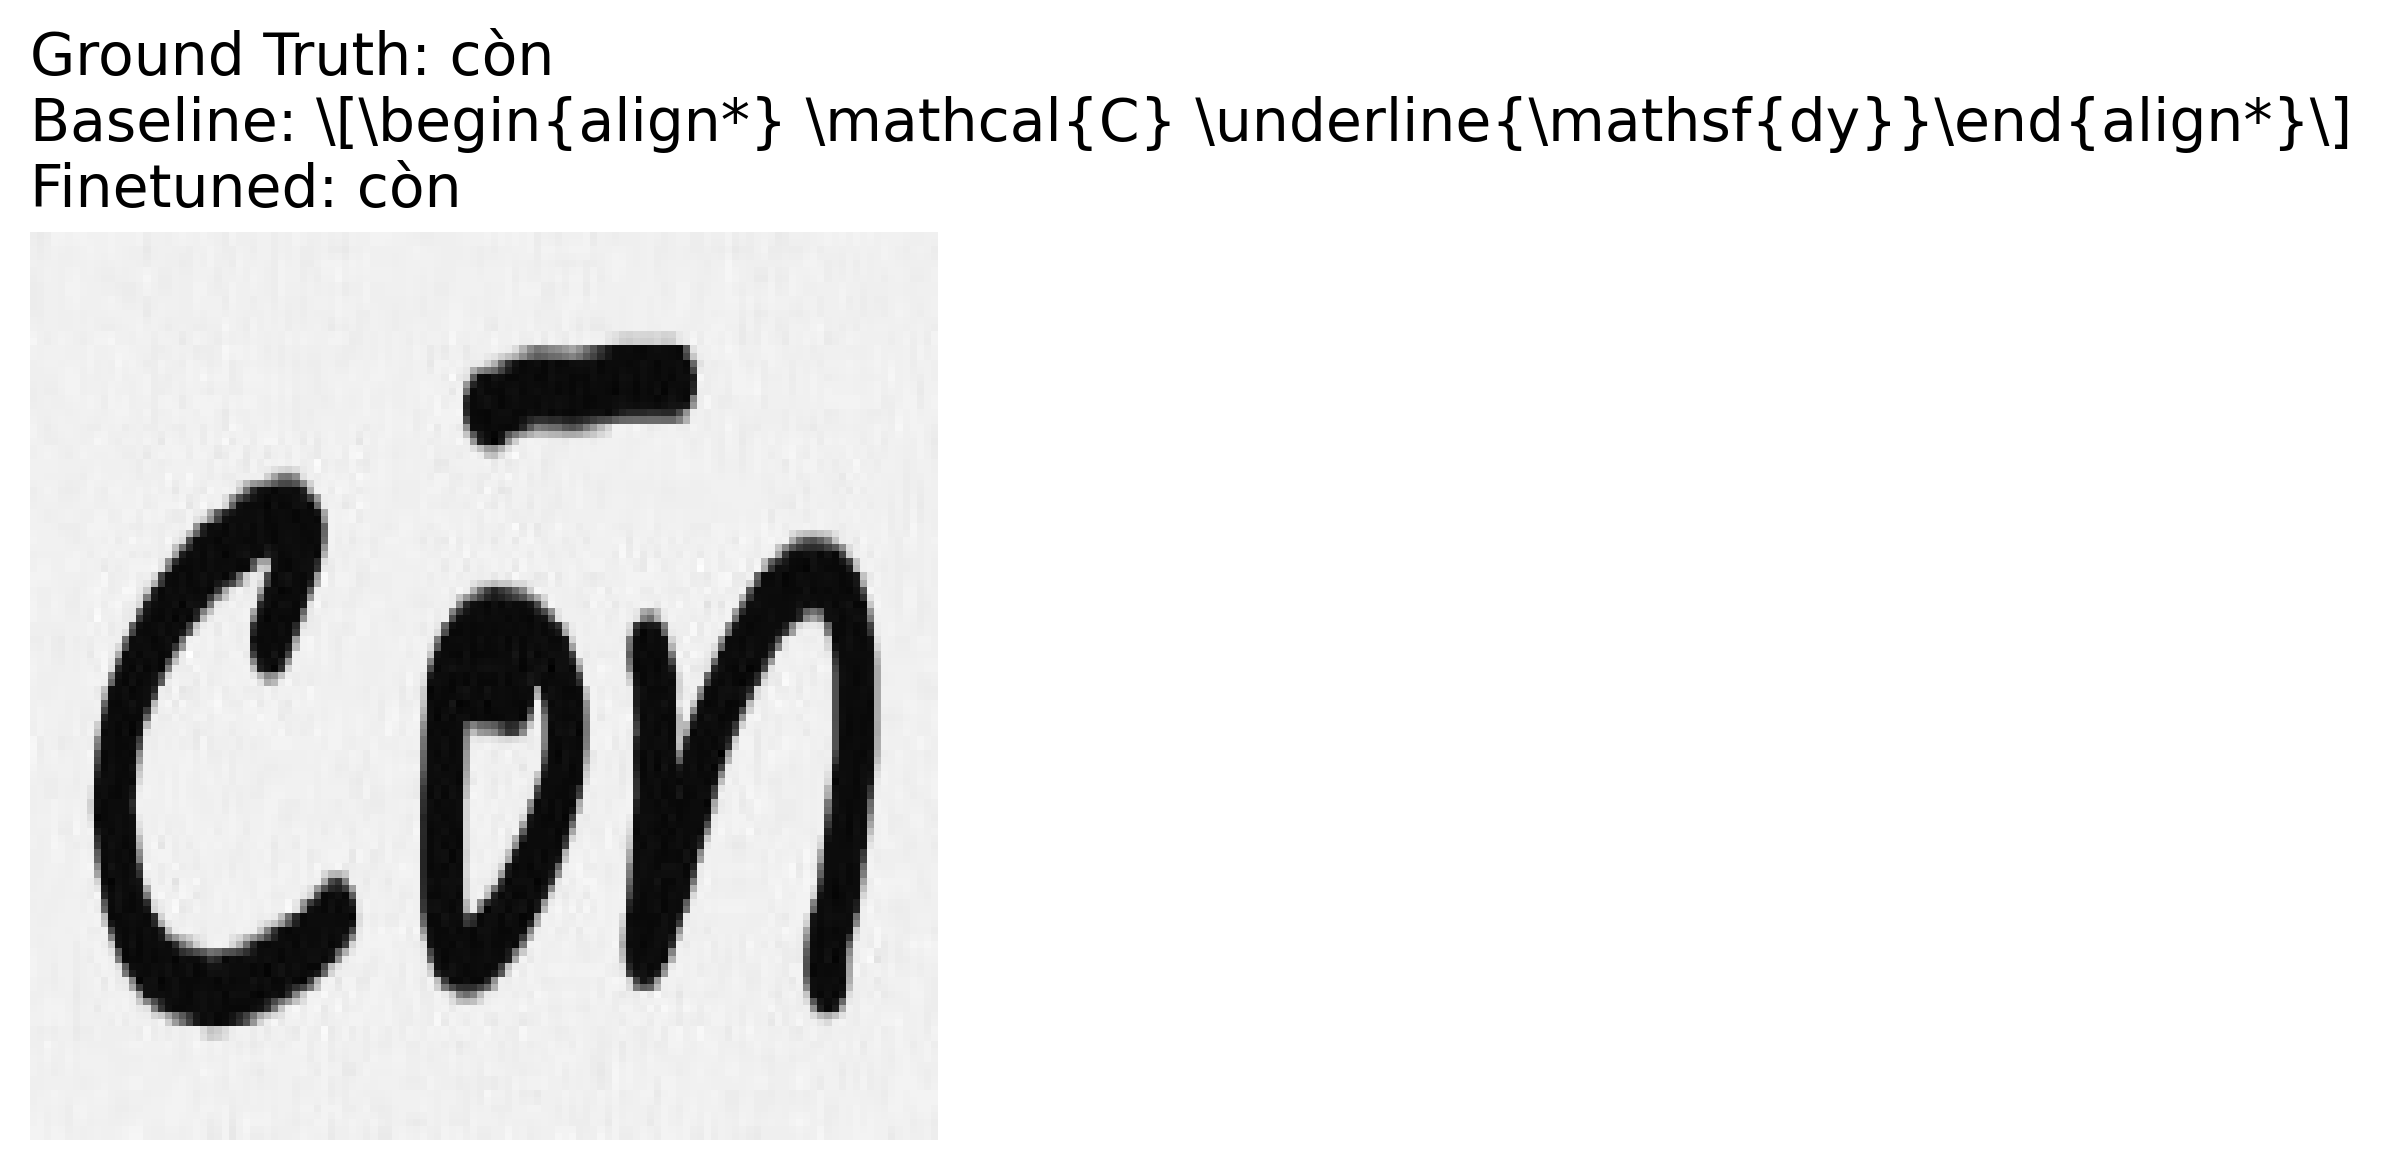
\includegraphics[width=0.8\linewidth]{img/results/improvement_example_3.png}
    \caption{Trường hợp cho thấy lỗi của mô hình Baseline được khắc phục hoàn toàn bởi mô hình Fine-tuned}
    \label{fig:improvement_3}
\end{figure}

\subsubsection{Các trường hợp lỗi còn tồn tại}
Mặc dù đạt kết quả khả quan, mô hình vẫn còn gặp một số lỗi trong các trường hợp khó:
\begin{itemize}
    \item \textbf{Nhầm lẫn các ký tự tương đồng:} Một số cặp ký tự có hình dạng viết tay rất giống nhau (như 'u' và 'n', 'h' và 'k') đôi khi vẫn bị nhận dạng sai nếu ngữ cảnh không rõ ràng.
    \item \textbf{Ảnh chất lượng thấp:} Đối với các ảnh quá mờ hoặc nhiễu nặng, mô hình có thể sinh ra các ký tự ảo (hallucination) hoặc bỏ sót ký tự.
\end{itemize}

Hình dưới đây là ví dụ điển hình về các trường hợp lỗi còn tồn tại liên quan đến nét viết tay quá tháu và nhầm lẫn ký tự:

\begin{figure}[H]
    \centering
    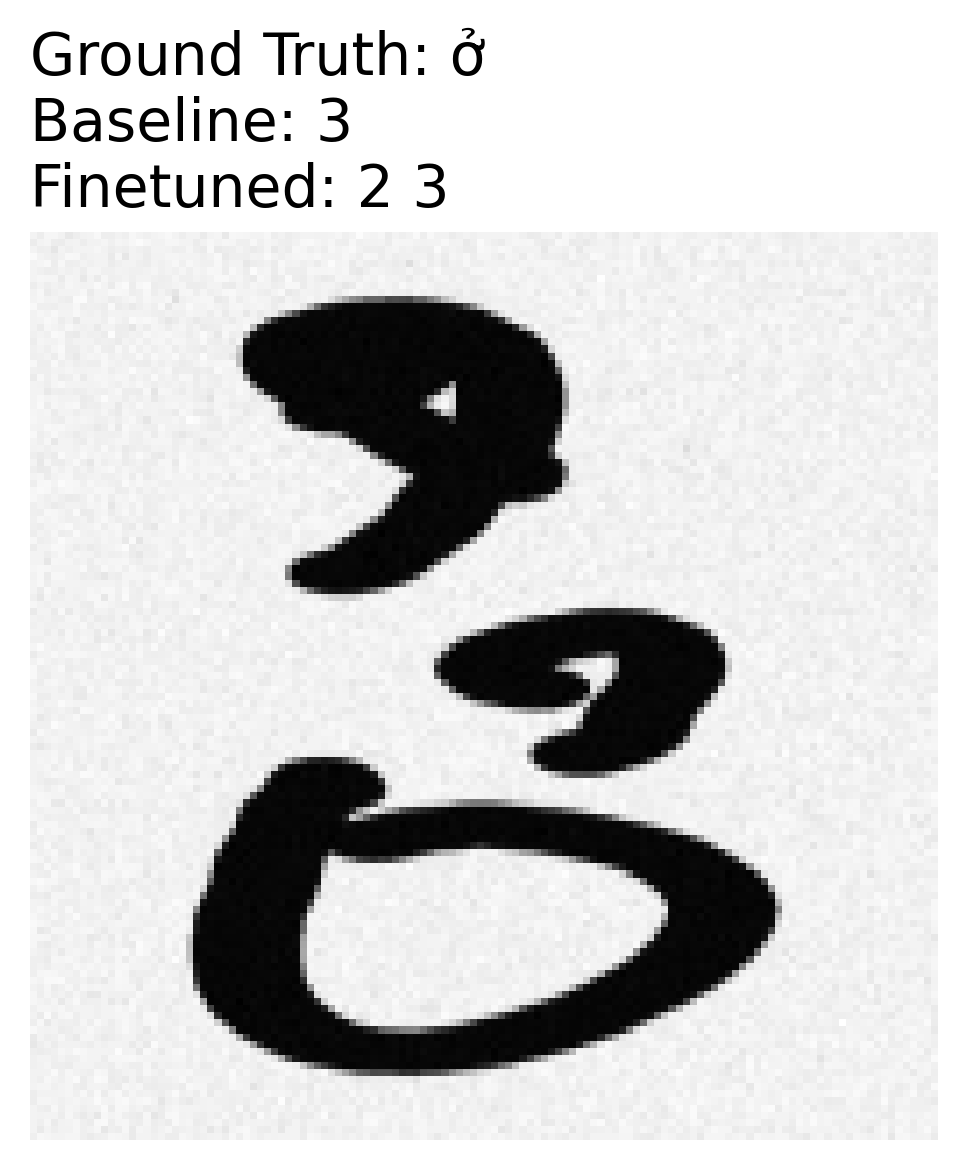
\includegraphics[width=0.4\linewidth]{img/results/worst_case_example_2.png}
    \caption{Trường hợp cho thấy mô hình fine-tuned vẫn gặp khó khăn với ảnh có chữ viết tay quá mờ và nét viết tháu. Hơn nữa, mô hình fine-tuned còn đạt được kết quả thấp hơn so với mô hình baseline trong ví dụ này.}
    \label{fig:worst_case_2}
\end{figure}
\section{Thảo luận}

Trong phần này, chúng tôi sẽ đánh giá mức độ cải thiện của mô hình, phân tích nguyên nhân dẫn đến kết quả đó, đồng thời thảo luận về các hạn chế còn tồn tại của dữ liệu, mô hình và quy trình huấn luyện.

\subsection{Đánh giá mức độ cải thiện}

Kết quả thực nghiệm cho thấy mô hình sau khi tinh chỉnh (Fine-tuned) đã đạt được sự cải thiện đáng kể so với mô hình cơ sở (Baseline) trên cả hai chỉ số CER và WER. Mức độ cải thiện này đặc biệt rõ rệt đối với các trường hợp chữ viết tay có nhiều dấu thanh phức tạp và nét viết tháu, nơi mà mô hình Baseline thường xuyên gặp lỗi. Sự giảm thiểu tỷ lệ lỗi không chỉ dừng lại ở mức độ nhận dạng ký tự đơn lẻ mà còn thể hiện ở khả năng khôi phục đúng các từ vựng tiếng Việt hoàn chỉnh.

\subsection{Phân tích nguyên nhân}

Sự cải thiện hiệu năng có thể được lý giải bởi các yếu tố chính sau:

\begin{itemize}
    \item \textbf{Kiến trúc Vision-Language ưu việt:} Khác với các hệ thống OCR truyền thống (CNN-RNN), DeepSeek-OCR kết hợp khả năng trích xuất đặc trưng hình ảnh mạnh mẽ với tri thức ngôn ngữ phong phú của LLM. Điều này cho phép mô hình không chỉ "nhìn" thấy nét chữ mà còn "hiểu" được ngữ cảnh, từ đó tự động sửa lỗi và điền khuyết các nét mờ dựa trên xác suất ngôn ngữ.
    \item \textbf{Hiệu quả của LoRA:} Kỹ thuật LoRA cho phép mô hình thích nghi nhanh chóng với miền dữ liệu chữ viết tay tiếng Việt mà không làm mất đi khả năng tổng quát hóa. Việc cập nhật trọng số có chọn lọc giúp mô hình tập trung học các đặc trưng cụ thể của bộ dữ liệu UIT-HWDB (như cách viết dấu, độ nghiêng) một cách hiệu quả.
    \item \textbf{Cơ chế xử lý ảnh động:} Việc sử dụng crop\_mode giúp mô hình bảo toàn độ phân giải cao của ảnh đầu vào, cho phép nhận diện rõ ràng các chi tiết nhỏ như dấu nặng, dấu hỏi - vốn là điểm yếu của các phương pháp nén ảnh về kích thước cố định.
\end{itemize}

Tuy nhiên, trong một số trường hợp hãn hữu, mô hình vẫn chưa đạt được độ chính xác tuyệt đối. Nguyên nhân chủ yếu đến từ sự nhập nhằng quá lớn trong nét viết tay của một số mẫu dữ liệu, khiến ngay cả con người cũng khó phân biệt nếu không có ngữ cảnh rộng hơn.

\subsection{Hạn chế của nghiên cứu}

Mặc dù đạt kết quả khả quan, nghiên cứu vẫn còn tồn tại một số hạn chế:

\subsubsection{Hạn chế về dữ liệu}
\begin{itemize}
    \item \textbf{Quy mô và độ đa dạng:} Bộ dữ liệu UIT-HWDB, mặc dù chất lượng, nhưng vẫn còn hạn chế về quy mô so với các bộ dữ liệu tiếng Anh hay tiếng Trung \cite{le2025surveyvietnamesedocumentanalysis}. Sự thiếu hụt các mẫu chữ viết tay từ các vùng miền khác nhau hoặc các phong cách viết "lạ" có thể làm giảm khả năng tổng quát hóa của mô hình trong thực tế.
    \item \textbf{Phạm vi văn bản:} Dữ liệu hiện tại chủ yếu tập trung ở cấp độ từ (word-level) và dòng ngắn. Mô hình chưa được kiểm chứng kỹ lưỡng trên các tài liệu nguyên trang (full-page) với bố cục phức tạp.
\end{itemize}

\subsubsection{Hạn chế về mô hình và huấn luyện}
\begin{itemize}
    \item \textbf{Tốc độ suy luận:} Do sử dụng kiến trúc Transformer lớn, tốc độ suy luận của DeepSeek-OCR chậm hơn đáng kể so với các mô hình chuyên biệt nhẹ (như PaddleOCR). Điều này là rào cản lớn cho các ứng dụng yêu cầu phản hồi thời gian thực.
    \item \textbf{Vấn đề ảo giác (Hallucination):} Là đặc tính cố hữu của các mô hình sinh (Generative Models), đôi khi mô hình có thể tự sinh ra các từ ngữ không có trong ảnh, đặc biệt khi ảnh đầu vào quá nhiễu.
    \item \textbf{Tài nguyên tính toán:} Quá trình huấn luyện, dù đã dùng LoRA, vẫn yêu cầu tài nguyên GPU đáng kể, gây khó khăn cho việc triển khai và tinh chỉnh liên tục trên các thiết bị hạn chế tài nguyên.
\end{itemize}

\subsection{Hướng phát triển}

Dựa trên các phân tích trên, chúng tôi đề xuất một số hướng nghiên cứu tiếp theo:

\begin{itemize}
    \item \textbf{Mở rộng dữ liệu:} Thu thập và tổng hợp thêm dữ liệu chữ viết tay đa dạng hơn, bao gồm cả các mẫu văn bản hành chính, đơn từ để tăng tính thực tế.
    \item \textbf{Tối ưu hóa mô hình:} Nghiên cứu các kỹ thuật lượng tử hóa (Quantization) và chưng cất tri thức (Knowledge Distillation) để giảm kích thước mô hình và tăng tốc độ suy luận mà không làm giảm quá nhiều độ chính xác.
    \item \textbf{Hậu xử lý chuyên sâu:} Kết hợp thêm các module kiểm tra chính tả hoặc ràng buộc ngữ pháp tiếng Việt chặt chẽ hơn ở đầu ra để hạn chế lỗi ảo giác.
\end{itemize}
\section{Kết luận}

Nghiên cứu này đã trình bày một phương pháp tiếp cận hiện đại cho bài toán nhận dạng chữ viết tay tiếng Việt bằng cách tinh chỉnh mô hình Vision-Language DeepSeek-OCR. Thông qua các thực nghiệm và đánh giá chi tiết, chúng tôi rút ra những kết luận chính sau:

\begin{itemize}
    \item \textbf{Hiệu quả của mô hình Vision-Language:} Việc kết hợp khả năng trích xuất đặc trưng hình ảnh với tri thức ngôn ngữ của LLM đã mang lại hiệu quả vượt trội. Mô hình không chỉ nhận dạng ký tự mà còn hiểu được ngữ cảnh, giúp giải quyết triệt để các thách thức đặc thù của tiếng Việt như hệ thống dấu thanh phức tạp và các nét viết tay biến dạng.
    
    \item \textbf{Tính khả thi của kỹ thuật LoRA:} Kỹ thuật tinh chỉnh thích nghi hạng thấp (LoRA) đã chứng minh được tính hiệu quả cao, cho phép huấn luyện một mô hình lớn trên tài nguyên phần cứng hạn chế mà vẫn đạt được độ chính xác ấn tượng. Đây là một hướng đi hứa hẹn cho việc phát triển các ứng dụng AI chuyên biệt với chi phí thấp.
    
    \item \textbf{Cải thiện so với Baseline:} Kết quả thực nghiệm trên bộ dữ liệu UIT-HWDB cho thấy mô hình sau khi tinh chỉnh đã giảm đáng kể tỷ lệ lỗi ký tự (CER) và tỷ lệ lỗi từ (WER) so với mô hình gốc, đặc biệt là trong các trường hợp chữ viết tháu và ảnh có chất lượng không đồng đều.
\end{itemize}

Tuy nhiên, nghiên cứu cũng nhận diện được những rào cản về tốc độ suy luận và sự phụ thuộc vào dữ liệu huấn luyện. Trong tương lai, chúng tôi sẽ tập trung vào việc tối ưu hóa kiến trúc để giảm độ trễ, đồng thời mở rộng bộ dữ liệu để bao phủ nhiều loại hình văn bản thực tế hơn, hướng tới việc xây dựng một hệ thống OCR tiếng Việt toàn diện và mạnh mẽ.

\section{Tài nguyên liên quan}
Phần này cung cấp thông tin về mã nguồn và các tài nguyên liên quan được sử dụng trong nghiên cứu. Mã nguồn của dự án được công khai trên GitHub để đảm bảo tính minh bạch và khả năng tái tạo kết quả.

\begin{itemize}
    \item \href{https://github.com/p1neapplechoco/Vietnamese-Deepseek-OCR}{GitHub Repository: Vietnamese-Deepseek-OCR}
    \item \href{https://github.com/nghiangh/UIT-HWDB-dataset}{GitHub Repository: UIT-HWDB Dataset}
\end{itemize}

Các kết quả cùng với mã nguồn của mô hình được cung cấp cùng với các notebook trong repository của bài báo cáo.

% References
\input{ref/ref.tex}

\end{document}